% 2019-09-16
%
% Header can be about me and past tense: I have done X Y Z
%
% Body should describe results in the present tense, normal technical style
%
% The end of a section may use self-cites, and those may use past tense to
%  say "I did ...."

My research to date has focused on
 understanding the performance challenges for natural
 and comparing natural to other approaches.
These efforts have led up to the above thesis question.
The performance studies motivate a combination of \tdeep{} and \tshallow{}
 types, and suggest methods to empirically validate the result.
The comparison studies provide a theoretical model for defining the
 combination and understanding its formal guarantees.

% others = their they
%
% mine = our we

% This section reviews my prior work and explains how each project contributes
%  to the thesis question.


\subsection{Performance Evaluation}

Migratory typing promises the ability to mix typed and untyped code.
A performance evaluation for a migratory typing system must, therefore,
 evaluate mixed-typed programs.\footnote{\shorturl{https://www.}{ccs.neu.edu/home/asumu/papers/stop15-tfgnvf.pdf}}

\citet{tfdfftf-ecoop-2015} present the first systematic evaluation
 of a mixed-typed language.
The paper applies a method to two fully-typed programs consisting of four
 modules; for each program, this method demands the generation and
 measurement of $2^4$ partially-typed configurations.
The paper tabulates the results of this evaluation in two lattices showing
 the fully-untyped configuration on the bottom and fully-typed on top
 (\figureref{fig:takikawa-lattice}),
 and thereby shows the running times a programmer
 might see if they added the same types in an arbitrary manner.
Using these lattices, the paper discusses the worst-case performance
 and the existence of bottom-up paths through the lattice that avoid slowdowns.

\begin{figure}[h]
  \begin{tabular}{c@{\qquad\qquad}c}
  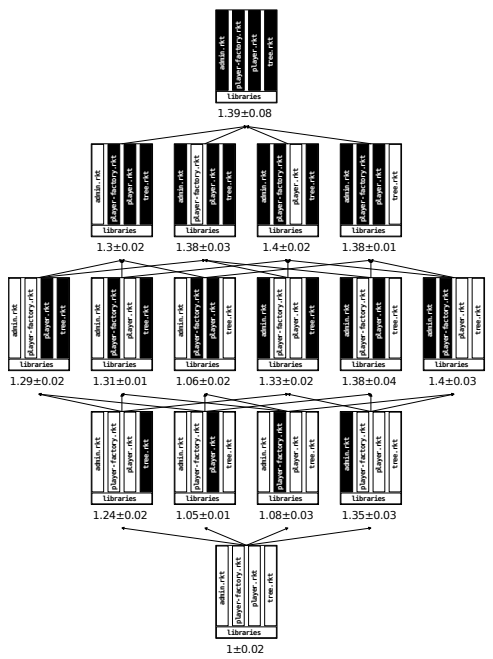
\includegraphics[width=0.30\columnwidth]{src/takikawa-lattice-acquire.png}
    &
  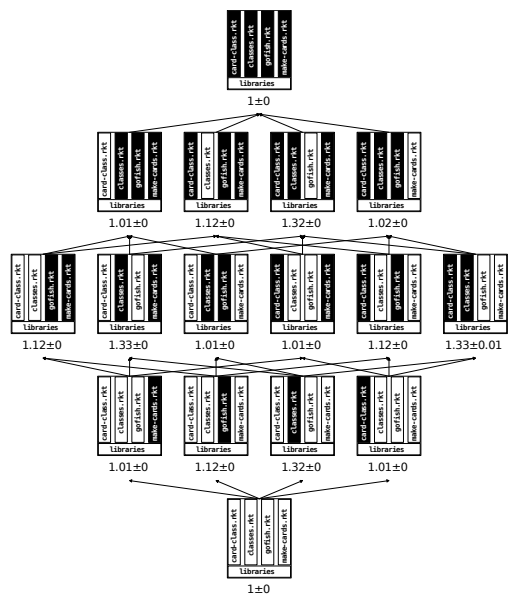
\includegraphics[width=0.30\columnwidth]{src/takikawa-lattice-gofish.png}
  \end{tabular}
  \caption{Performance results for two Typed Racket programs~\cite{{tfdfftf-ecoop-2015}}}
  \label{fig:takikawa-lattice}
\end{figure}

The method clearly needs further refinement; a lattice presents a lot
 of information, but does little to convey insights.
Furthermore, the exhaustive approach to data collection cannot handle large
 programs.
To summarize, the method raises at least three questions of size and scale:
 \begin{itemize}
   \item Is there a concise way to summarize the performance of a program?
   \item Can the method compare different implementations of migratory typing?
   \item Can the method be adapted to programs with a large number (+20) of configurations?
 \end{itemize}
My work on performance evaluation developed answers to these questions.


\subsubsection{Summarizing Performance}

% NOTE
%The typical ``summary statistics'' of mean, median, min, and max were also a
% poor fit; although worst-case performance could be terrible
% (\figureref{fig:max-overhead}), there is no guarantee that a programmer
% will actually encounter the worst case.

%Turing's negative answer to the halting problem tells us that a computer
% program cannot tell the difference between an infinite running time and
% a very large one.

Our method of summarizing the performance in an exponentially-large set
 is based on a fundamental law of software development:
 all programs that are not ``fast enough'' are equally worthless.

\citet{tfgnvf-popl-2016} use this relevance law to summarize the performance
 of a migratory typing system.
If a configuration meets a fixed performance requirement, then it is good.
Otherwise it is worthless.
With this binary classification method, the performance of a mixed-typed
 program may be summarized with a ratio; namely,
 the proportion of good configurations.
Likewise, a sequence of benchmarks may be summarized with a sequence of ratios.
These ratios can help software developers assess the performance risk of
 migratory typing.

Technically, \citet{tfgnvf-popl-2016} call a configuration \deliverable{D}
 if its running time is no more than $D$x slower than the baseline performance
 with no migratory typing.\footnote{In Racket, the fully-untyped configuration
 is an appropriate baseline. In Reticulated Python, the fully-untyped configuration
 run via Python (not via Reticulated) is an appropriate baseline~\cite{gm-pepm-2018}.}
Given a positive number $D$, the proportion of \deliverable{D} configurations
 is exactly the proportion of ``good'' configurations described above.

The paper accommodates varying notions of good performance by combining the
 results for $D$ between $1$ and $20$ into a plot.
The $x$-axis of such a plot ranges over values of $D$.
The $y$-axis ranges over the number (or percent) of configurations.
\Figureref{fig:snake-popl}, on the left-hand side, presents an example
 for a program with eight modules.
The key takeaway is that the plot answers an important question and does
 not require an exponential amount of space.

\begin{figure}[h]
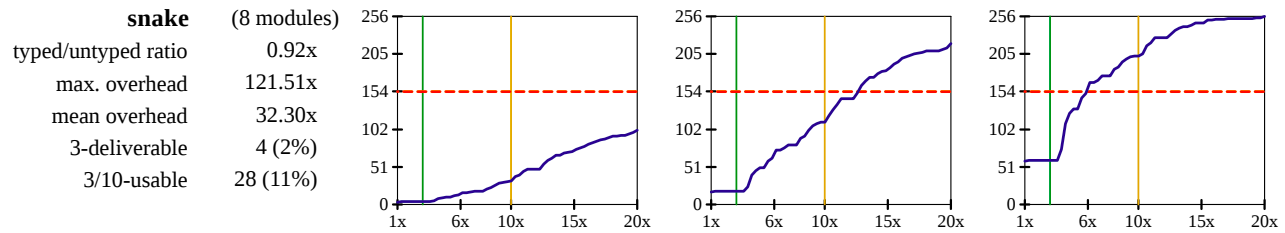
\includegraphics[width=0.96\columnwidth]{src/snake-popl.png}
\caption{Counting \deliverable{D} configurations in the \bm{snake}
         benchmark~\cite{tfgnvf-popl-2016}. The $x$-axis ranges over $D$ values;
         the vertical lines mark $D=3$ and $D=10$.
         The $y$-axis counts configurations; the dashed horizontal line marks
         $60$\% of all configs.
         The thick blue line is the number of \deliverable{x} configs.}
\label{fig:snake-popl}
\end{figure}

Variations on the \deliverable{D} metric can answer similar questions
 about a mixed-typed program.
For example, the two other plots in \figureref{fig:snake-popl}
 relax the metric to allow 1 (middle plot) and 2 (right plot) extra type
 conversion steps.
In this case, one conclusion supported by the right-most plot is that
 if a $10$x slowdown is acceptable and the client is willing to add types
 to at most two extra modules, then 80\% of the configurations can reach
 an acceptable state.
Once again the key takeaway is not the particular conclusion,
 but the fact that the method helps answer useful questions.


\subsubsection{Comparing Implementations}
% Can the method compare different implementations of migratory typing?

The \deliverable{D} metric enables comparisons of different migratory
 typing systems.
If there are two languages that can execute the same program,
 then the language with better performance is the one that maximizes the
 number of \deliverable{D} configurations.
The difference may be plotted by drawing two curves on the same
 axes.

\citet{gtnffvf-jfp-2019} use this observation to compare three versions
 of Racket: v6.2, v6.3, and v6.4.
Racket~v6.3 contains a few improvements inspired by the performance
 evaluation of Racket v6.2~\cite{tfgnvf-popl-2016}.
Racket~v6.4 contains many more changes:
 it inlines the contract checks for simple typed functions,
 validates struct predicates with a first-order check (instead of a higher-order wrapper),
 and reduces the memory overhead of contract in general.
\Figureref{fig:snake-jfp} shows the effect of these changes on one benchmark.
The curve for version 6.4 lies above the others, meaning the percent of
 \deliverable{D} configurations is increased for every value of $D$ along
 the $x$ axis.

\begin{figure}[ht]
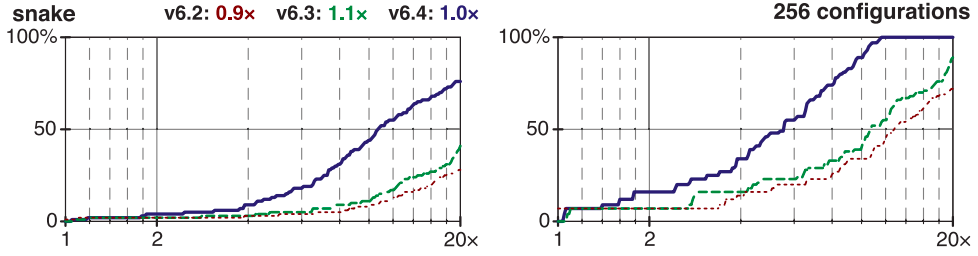
\includegraphics[width=0.8\columnwidth]{src/snake-jfp.png}
\caption{Comparing performance across three versions of Typed Racket; the right plot allows one type conversion step}
\label{fig:snake-jfp}
\end{figure}

These plots appear in related work:\footnote{\citet{kat-pldi-2019} plot the
 \deliverable{D} configurations in Typed Racket alongside a count based on
 the overhead of a new language, Grift, relative to Racket.
 The latter is not the \deliverable{D} metric because removing all typse from
 a Grift program does not produce a Racket program.}
\citet{bbst-oopsla-2017} demonstrate the benefits of adding a tracing JIT compiler to Typed Racket;
\citet{fgsfs-oopsla-2018} measure the impact of collapsible higher-order contracts; and
\citet{gf-icfp-2018} compare Typed Racket to a prototype implementation of transient type checks.


\subsubsection{Scaling the Method}
% Can the method be adapted to programs with a large number (+20) of configurations?

\citet{gm-pepm-2018} adapt the method to evaluate the performance of Reticulated
 Python.
By contrast to Typed Racket, Reticulated allows optional type annotations at
 a fine granularity.
Every function/method parameter, function return type, and class field may
 be optionally annotated.
Unfortunately for the exhaustive method, this freedom means that relatively
 small programs may have a huge number of configurations---counting
 the proportion of \deliverable{D} is impractical for a class with 20 fields.

The paper demonstrates, however, that a linear number of random samples can
 approximate the true number of good configurations.
Intuitively, the result is that the overhead experienced by $N$ developers
 provides useful information for the next one to add types to the same program.

To approximate the proportion of \deliverable{D} configurations,
 first select $s$ configurations uniformly at random and count the
 proportion of \deliverable{D} configurations in this sample.
Repeat for $r$ samples to build a set of proportions.
Use the set to build a confidence interval, and finally interpret the
 confidence interval to approximate the true deliverable configurations.

\citet{gm-pepm-2018} perform an experiment in which $r=10$ is a constant
 and $s = 10 * (F + C)$ is linear in the number of functions $F$ and classes
 $C$ in a benchmark.
For six benchmarks with 12 to 17 functions and classes each,
 they generate six 95\%~confidence intervals.
To validate these results, they collect the running time of every configuration
 in which: any function/method may be typed or untyped, and the set of fields
 for any class may be typed or untyped.
Note that this is fewer configurations than Reticulated allows.
% TODO more to say?
As \figureref{fig:sampling} shows, the confidence intervals provide a tight
 bound on the ground truth.

\begin{figure}[h]
  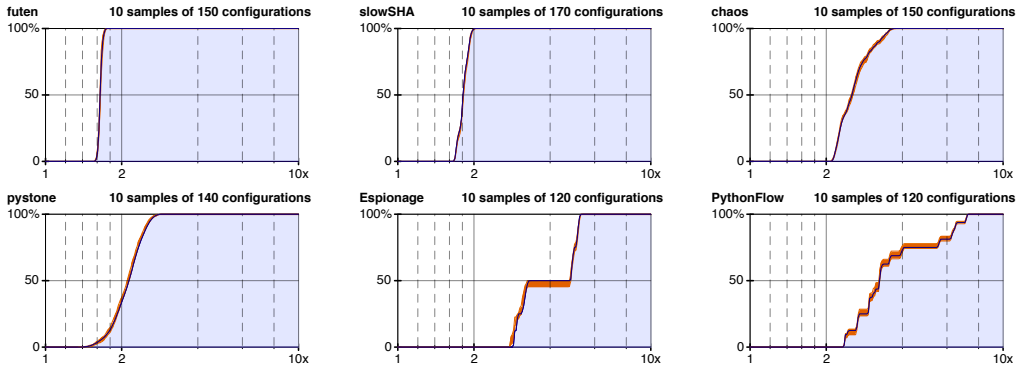
\includegraphics[width=\columnwidth]{src/sampling.png}
  \caption{Thin blue lines plot \deliverable{D} configurations; thick brown lines plot 95\% confidence intervals}
  \label{fig:sampling}
\end{figure}

\citet{gtnffvf-jfp-2019} also validate the sampling method on Typed Racket
 programs.
They use the same number of samples and same linear sample size, and find
 that the intervals yield tight approximations.

%Thanks to the approximation method, \cite{gm-pepm-2018} evaluate three programs
% with 19, 34, and 79 typed units each.


\subsubsection{Benchmark Suite}

\citet{gtnffvf-jfp-2019} formally introduce a suite of mixed-typed benchmark
 programs.
The benchmarks are available online\footnote{\shorturl{https://}{docs.racket-lang.org/gtp-benchmarks/}}
 and have been used to validate other work on Typed Racket~\cite{gf-icfp-2018,bbst-oopsla-2017}.
% also Cameron (in submission) + Lukas (in submission)


\subsection{Comparative Model}

Models of migratory typing systems come in many varieties---often because
 the models reflect a proof-of-concept implementation~\cite{bat-ecoop-2014,wnlov-popl-2010,mt-oopsla-2017,vss-popl-2017,tf-popl-2008}.
 % TODO cite many more
These models share the common goal of mixing static and dynamic typing,
 but realize the goal with different formalizations.
Unfortunately, the diversity makes it difficult to compare the
 properties satisfied by each.

\citet{clzv-ecoop-2018} provide one unified model via a typed language,
 \kafka{}, that can express different methods of enforcing types.
The paper uses \kafka{} as a target language for four translations from
 a mixed-typed surface language; the translations represent natural,
 concrete, erasure, and transient.
The paper illustrates the differences between semantics with examples,
 but does not provide a formal characterization.

For my work on comparing styles of migratory typing, we developed
 a model that expresses styles as different semantics
 for a common surface language.
The common model enabled fair comparisons of properties
 such as type soundness and complete monitoring.
Additionally, the model facilitated the design of new semantics for migratory
 typing.
% Need to mention other things? This paragraph should lead into the subsections

\subsubsection{A Spectrum of Type Soundness}

% developed model, (1) what are boundaries (2) what are checks
% implemented for TR
% - same method! aha
% - 

\citet{gf-icfp-2018} introduce a model to compare natural, erasure, and
 transient migratory typing as different semantics for a common surface
 language.
The common language is a mixed-typed system in the style of \citet{mf-toplas-2009};
 it syntactically combines a statically-typed language with a dynamically-typed
 language via boundary terms.
For example, the typed expression
 $(\eapp{(\edyn{(\tarr{\tint}{\tint})}{\efun{\svar_0}{\svar_0}})}{2})$
 applies a dynamically-typed value to a statically-typed input.
The type annotation $(\tarr{\tint}{\tint})$ helps the static type checker
 validate the application and may affect the behavior of a semantics.

In this model, the differences between type-enforcement strategies
 come about as different behaviors for boundary terms.
The natural semantics strictly enforces types at a dynamic-to-static
 boundary.
Incoming higher-order values get wrapped in a proxy to monitor their
 behavior; other values receive an exhaustive check (\figureref{fig:nt-boundary}, left).
At a static-to-dynamic boundary, the natural approach wraps outgoing
 higher-order values to protect against future untyped inputs.
Since higher-order values may appear within first-order data structures,
 the latter require a traversal.

The erasure semantics treats boundary terms as a no-op.
Any value may cross any boundary.

The transient semantics enforces boundary terms with tag checks (\figureref{fig:nt-boundary}, right);
 however, it also treats elimination forms in typed code as boundaries.
A dynamic-to-static boundary checks that the top-level shape of an incoming
 value matches the outermost constructor of the expected type.
A static-to-dynamic boundary lets any value cross; if typed code satisfies a
 tag-level soundness guarantee, then such values are certain to match the
 outermost constructor of the expected type.
Transient achieves this guarantee by guarding every elimination form in typed
 code with a dynamic-to-static check.
Thus if the untyped value $\epair{{-2}}{{0}}$ enters typed code via a
 $(\tpair{\tnat}{\tnat})$ boundary and typed code projects the first element
 of the pair expecting a nonnegative integer, a runtime check halts the program.

% note that checks overapproximate, but succeed without wrappers?

\begin{figure}[ht]
  \begin{minipage}[t]{0.5\columnwidth}
 \fbox{$\DNsym : \tpair{\stype}{\svalue} \rightarrow \svalue \cup \serror$}\\
  \(\begin{mfarray}
    \fDN{\tarr{\stype_0}{\stype_1}}{\svalue_0}
    & = &
    \emon{\tarr{\stype_0}{\stype_1}}{\svalue_0}
    \\\sidecond{if $\svalue_0$ is a function}
    \\
    \fDN{\tpair{\stype_0}{\stype_1}}{\epair{\svalue_0}{\svalue_1}}
    & = &
    \epair{\edyn{\stype_0}{\svalue_0}}{\edyn{\stype_1}{\svalue_1}}
    \\
    \fDN{\tint}{\sint_0}
    & = &
    \sint_0
    \\
    \fDN{\tnat}{\sint_0}
    & = &
    \sint_0
    \\\sidecond{if $0 \leq \sint_0$}
    \\
    \fDN{\stype_0}{\svalue_0}
    & = &
    \serror
    \\\sidecond{otherwise}
  \end{mfarray}\)

  \fbox{$\SNsym : \tpair{\stype}{\svalue} \rightarrow \svalue \cup \serror$}\\
  \(\begin{mfarray}
    \fSN{\tarr{\stype_0}{\stype_1}}{\svalue_0}
    & = &
    \emon{(\tarr{\stype_0}{\stype_1})}{\svalue_0}
    \\\sidecond{if $\svalue_0$ is a function}
    \\
    \fSN{\tpair{\stype_0}{\stype_1}}{\epair{\svalue_0}{\svalue_1}}
    & = &
    \epair{\esta{\stype_0}{\svalue_0}}{\esta{\stype_1}{\svalue_1}}
    \\
    \fSN{\stype_0}{\svalue_0}
    & = &
    \svalue_0
    \\\sidecond{otherwise}
  \end{mfarray}\)
  \end{minipage}\begin{minipage}[t]{0.5\columnwidth}
  \fbox{$\DTsym : \tpair{\stype}{\svalue} \rightarrow \svalue \cup \serror$}\\
  \(\begin{mfarray}
    \fDT{\tarr{\stype_0}{\stype_1}}{\svalue_0}
    & = &
    \svalue_0
    \\\sidecond{if $\svalue_0$ is a function}
    \\
    \fDT{\tpair{\stype_0}{\stype_1}}{\svalue_0}
    & = &
    \svalue_0
    \\\sidecond{if $\svalue_0$ is a pair}
    \\
    \fDT{\tint}{\sint_0}
    & = &
    \sint_0
    \\
    \fDT{\tnat}{\sint_0}
    & = &
    \sint_0
    \\\sidecond{if $0 \leq \sint_0$}
    \\
    \fDT{\stype_0}{\svalue_0}
    & = &
    \serror
    \\\sidecond{otherwise}
  \end{mfarray}\)

  \fbox{$\STsym : \tpair{\stype}{\svalue} \rightarrow \svalue \cup \serror$}\\
  \(\begin{mfarray}
    \fST{\stype_0}{\svalue_0}
    & = &
    \svalue_0
  \end{mfarray}\)
  \end{minipage}

  \caption{Boundary checks for natural (left) and transient (right)}
  \label{fig:nt-boundary}
\end{figure}

% ... spectrum of soundness
These three methods of enforcing type boundaries lead to three different
 semantics for surface programs.
One may compare the results of running one program via the three semantics,
 and one may formulate theorems that characterize general differences.
The models therefore serve as a tool for language analysis.
\citet{gf-icfp-2018} demonstrate one analysis by proving three pairs of type
 soundness theorems for the semantics.
For typed contexts, these theorems roughly guarantee that:
 the natural semantics can only yield values that fully match the expected type;
 the erasure semantics can yield any value;
 and the transient semantics can only yield values with a tag that matches
 the outermost constructor of the expected type.
Sibling theorems describe the behavior of untyped code.

Additionally, the models serve as a tool for language design.
One may develop a new semantics by proposing a new strategy for checking
 the boundaries between typed and untyped components.
\citet{gf-icfp-2018} present two such variants of the natural semantics,
 dubbed co-natural and forgetful.
In short, these two bridge the gap between natural and transient.
Co-natural allocates wrappers for all kinds of structured data---not only
 higher-order values---and thereby reduces the amount of checking at a boundary
 to a tag check.
Forgetful extends co-natural; if a wrapped value reaches a boundary, a new
 wrapper replaces the existing one.

%Both co-natural and forgetful provide a type soundness guarantee that resembles
% the guarantee for natural, but enforce fewer type guarantees.
%\citet{gf-icfp-2018} prove an errors-inequality theorem but say no more
 
%With the models as a guide, we implemented a transient prototype for a
% functional subset of Typed Racket~\cite{gf-icfp-2018}.
%The prototype enabled a systematic comparison of the natural and transient
% styles; starting with one suite of surface-language programs, we ran
% each under two semantics.
%
%The results of the evaluation confirmed our earlier conjectures.
%Natural may have abysmal performance on heavily-mixed programs,
% but performs well when all but a few modules are typed.
%Transient rarely slows a program by 10x, but its cost increases with the
% quantity of type annotations.
%In a fully-typed program, natural is likely the best choice;
% in partially typed programs, however, transient can have far better
% performance.



\subsubsection{Honest vs. Lying Types}
% what did we learn?

The model makes it clear that the semantic choices affect behavior.
The differences are not explained by type soundness; can demonstrate
 with a compromise semantics (co-natural, amnesic).

% cannot trust types example?

To fix, adapted insights from the world of higher-order contracts to migratory
 typing.
A contract system satisfies complete monitoring if it is possible to attach
 a contract to every channel of communication between parties.
The practical significance is that complete monitoring offers an explanation
 for every contract violation; the system can pinpoint the faulty boundary.

A mixed-typed language satisfies complete monitoring if every channel of
 communication between typed and untyped components is protected with
 appropriate type-checks.
This means that programmers can trust the types,
 whether they work on typed or untyped code;
 a system that satisfies complete monitoring gives types an indefinite extent.

Complete monitoring formalizes the intuitive notions of honest and lying types.
Well-monitored types cannot lie.

On the other hand, complete monitoring is apparently expensive.

Now that we can state complete monitoring theorems, we can ask whether a combined
system satisfies them.


\subsubsection{Interlude: User Study}

\citet{tgpk-dls-2018} leverage the common understanding from the model
 to create a survey about different gradual typing semantics.

The survey follows a mystery languages outline.
Participants are faced with a series of programs written in a hypothetical
 syntax.
Each program comes with two to three possible outcomes.
The question is whether each outcome is liked and/or expected; to be precise
 there are four choices: liked and expected, dislike and expected,
 liked and unexpected, dislike and unexpected.
% (Few questions received zero responses in a category.)

The survey demonstrates that the model is useful.
The responses suggest a preference for honest types.

% TODO can segue into "need characterization"


